% Chapter Template

\chapter{Biometric System Evaluation} % Main chapter title

\label{Chapitre 4.1} % Change X to a consecutive number; for referencing this chapter elsewhere, use \ref{ChapterX}

\lhead{ \emph{Biometric System Evaluation}} % Change X to a consecutive number; this is for the header on each page - perhaps a shortened title

%----------------------------------------------------------------------------------------
%	SECTION 1
%----------------------------------------------------------------------------------------
\section{Scores distribution}

Le but de cet exercice est d'analyser les performance d'un système biométrique à 2 classes. Ce système possède deux listes de scores : "genuine" et "impostors".  \\

Voilà le résulat de la fonction "hist()" mise en forme avec matlab : 

\begin{center} 
\hspace{15cm}
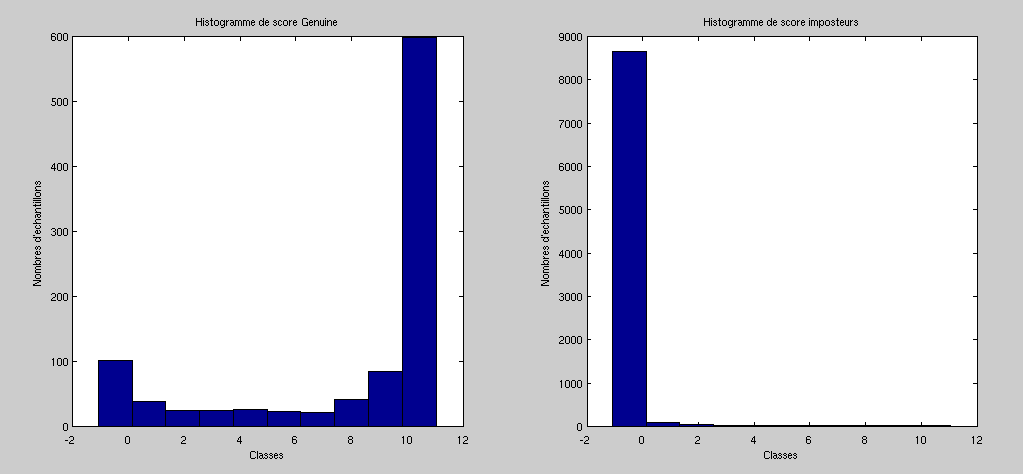
\includegraphics[width=15cm]{Histo.png}
\end{center}
\vspace{1cm} 

On peut remarquer le score "genuine" (à gauche) et score "impostors" (à droite) ont une répartitions des scores bien distincte. Toutefois, on peut remarquer qu'il a un petit recouvrement des zones. Cela signifie que l'on aura probablement des quelques fausse réjections ou même fausses acceptations selon le seuil appliqué.
\pagebreak


\section{Biometric performance curves}

Cette partie de cet exercice consistait à tracer différents graphique de performance du système biométrique étudié. 

Voilà les courbes FA(T) et FR(T) :

\begin{center} 
\hspace{15cm}
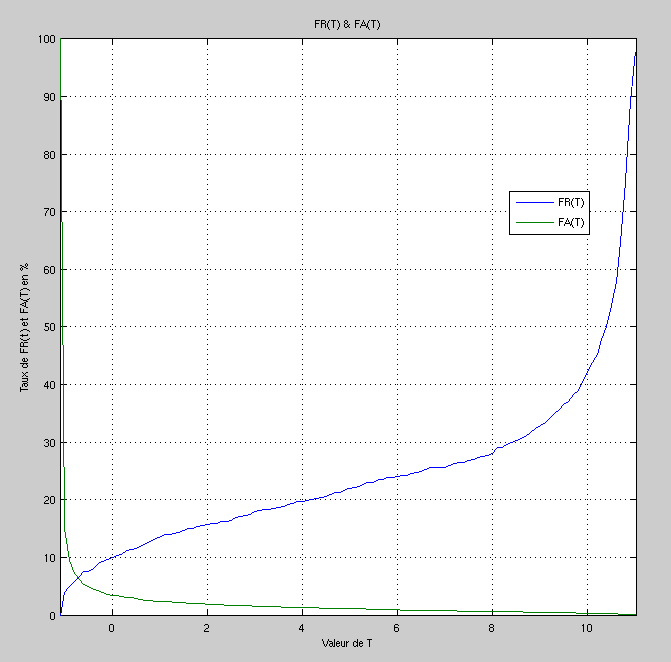
\includegraphics[width=15cm]{fa_fr_t.png}
\end{center}
\vspace{1cm} 

On remarque (même que c'est assez logique) que plus "T" est petit, plus le taus de fausses acceptations augmente (on accepte tout le monde). On voit aussi que plus notre "T" est grand, plus on aura tendance à refuser le vrai utilisateurs du système. Le but est d'essayer de trouver un bon compromis, entre refuser un utilisateur ou accepter un imposteur.\\

\textit{Remarques :} On peut observer un recouvrement des deux courbes, ce que l'on avait aussi observé sur les histogrammes.
\pagebreak


Voilà maintenant la courbe ROC linéaire :

\begin{center} 
\hspace{15cm}
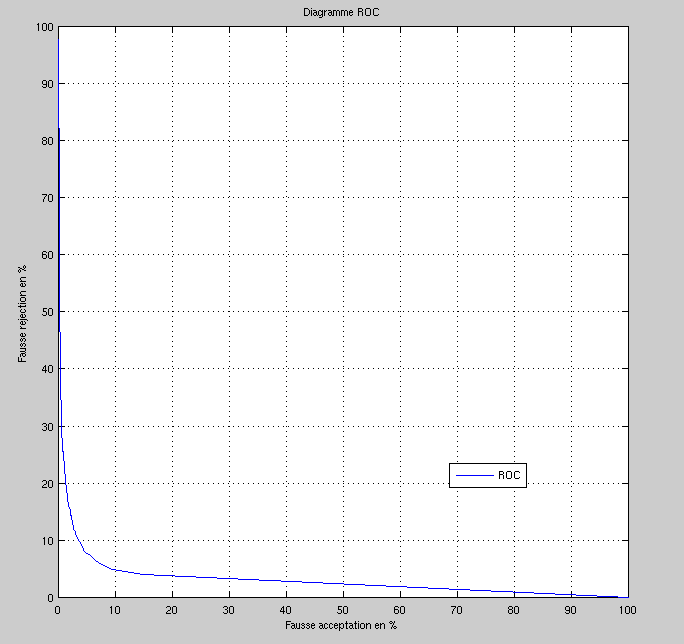
\includegraphics[width=15cm]{ROC.png}
\end{center}
\vspace{1cm} 

Cette fois on à représenté le taux probable de fausses réjections et fausses acceptations. Pus le coude est proche de l'origine, meilleur sera notre système. 

\pagebreak
Pour terminer, voilà la courbe ROC logarithmique, nommée DET :

\begin{center} 
\hspace{15cm}
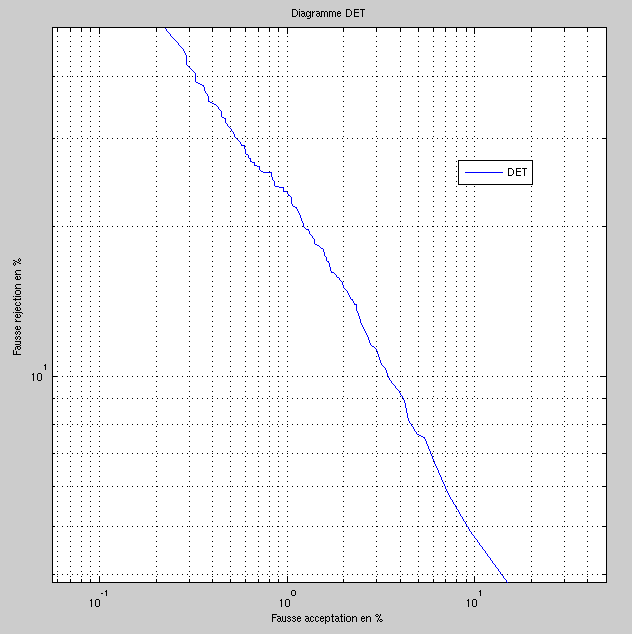
\includegraphics[width=8cm]{DET.png}
\end{center}
\vspace{1cm} 

Nous n'avons malheureusement pas compris pourquoi cette courbe ne ressemble pas à celle proposé par le petit logiciel Java fourni sur "Cyberlearn". Pourtant les autre courbes, elles paraissent juste ! Voici ce  que nous aurions du obtenir :

\begin{center} 
\hspace{15cm}
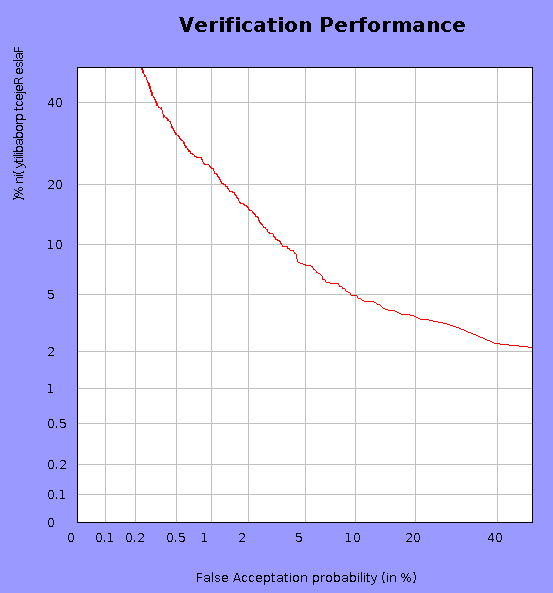
\includegraphics[width=8cm]{DET_J.png}
\end{center}
\vspace{1cm} 

Peut-être serait-ce uniquement une histoire d'échelle ? Nous ne savons pas... Le fait est que nous nous sommes arrêtés ici pour cet exercice (par manque de résultats et de temps). 
